\documentclass[14pt]{extbook}
\usepackage{multicol, enumerate, enumitem, hyperref, color, soul, setspace, parskip, fancyhdr} %General Packages
\usepackage{amssymb, amsthm, amsmath, latexsym, units, mathtools} %Math Packages
\everymath{\displaystyle} %All math in Display Style
% Packages with additional options
\usepackage[headsep=0.5cm,headheight=12pt, left=1 in,right= 1 in,top= 1 in,bottom= 1 in]{geometry}
\usepackage[usenames,dvipsnames]{xcolor}
\usepackage{dashrule}  % Package to use the command below to create lines between items
\newcommand{\litem}[1]{\item#1\hspace*{-1cm}\rule{\textwidth}{0.4pt}}
\pagestyle{fancy}
\lhead{Makeup Progress Quiz 3}
\chead{}
\rhead{Version C}
\lfoot{1648-1753}
\cfoot{}
\rfoot{Summer C 2021}
\begin{document}

\begin{enumerate}
\litem{
Determine the domain of the function below.\[ f(x) = \frac{6}{30x^{2} -7 x -15} \]\begin{enumerate}[label=\Alph*.]
\item \( \text{All Real numbers.} \)
\item \( \text{All Real numbers except } x = a \text{ and } x = b, \text{ where } a \in [-1.42, -0.37] \text{ and } b \in [0.6, 1.37] \)
\item \( \text{All Real numbers except } x = a, \text{ where } a \in [-1.42, -0.37] \)
\item \( \text{All Real numbers except } x = a \text{ and } x = b, \text{ where } a \in [-16.01, -14.82] \text{ and } b \in [29.58, 30.49] \)
\item \( \text{All Real numbers except } x = a, \text{ where } a \in [-16.01, -14.82] \)

\end{enumerate} }
\litem{
Solve the rational equation below. Then, choose the interval(s) that the solution(s) belongs to.\[ \frac{-63}{-35x + 14} + 1 = \frac{-63}{-35x + 14} \]\begin{enumerate}[label=\Alph*.]
\item \( x_1 \in [-0.3, 1] \text{ and } x_2 \in [-3.6,1.4] \)
\item \( x_1 \in [-0.8, 0] \text{ and } x_2 \in [-3.6,1.4] \)
\item \( \text{All solutions lead to invalid or complex values in the equation.} \)
\item \( x \in [0.4,1.4] \)
\item \( x \in [-0.8,0] \)

\end{enumerate} }
\litem{
Choose the equation of the function graphed below.
\begin{center}
    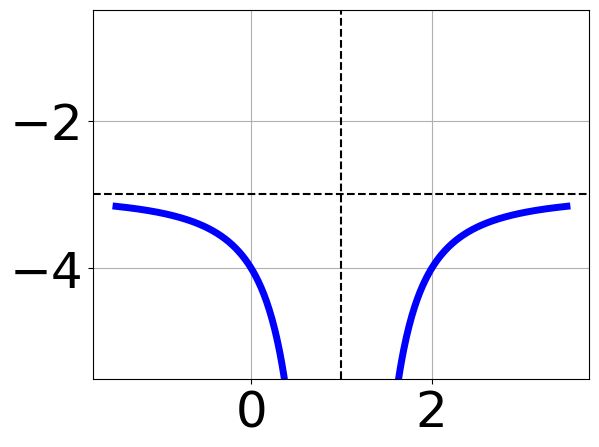
\includegraphics[width=0.5\textwidth]{../Figures/rationalGraphToEquationCopyC.png}
\end{center}
\begin{enumerate}[label=\Alph*.]
\item \( f(x) = \frac{-1}{x + 1} + 4 \)
\item \( f(x) = \frac{-1}{(x + 1)^2} + 4 \)
\item \( f(x) = \frac{1}{x - 1} + 4 \)
\item \( f(x) = \frac{1}{(x - 1)^2} + 4 \)
\item \( \text{None of the above} \)

\end{enumerate} }
\litem{
Choose the graph of the equation below.\[ f(x) = \frac{1}{x - 2} + 1 \]\begin{enumerate}[label=\Alph*.]
\begin{multicols}{2}\item 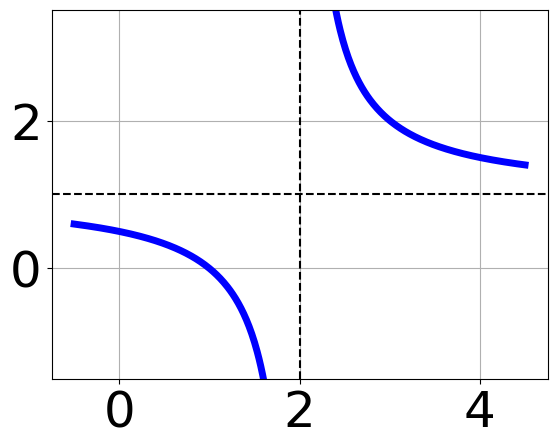
\includegraphics[width = 0.3\textwidth]{../Figures/rationalEquationToGraphCopyAC.png}\item 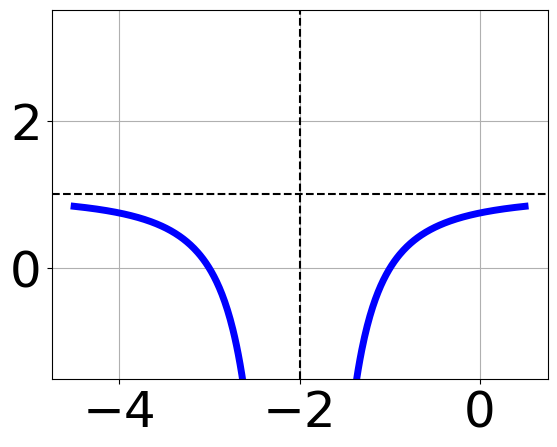
\includegraphics[width = 0.3\textwidth]{../Figures/rationalEquationToGraphCopyBC.png}\item 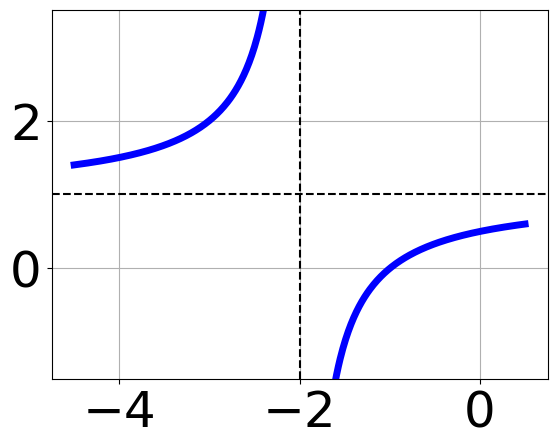
\includegraphics[width = 0.3\textwidth]{../Figures/rationalEquationToGraphCopyCC.png}\item 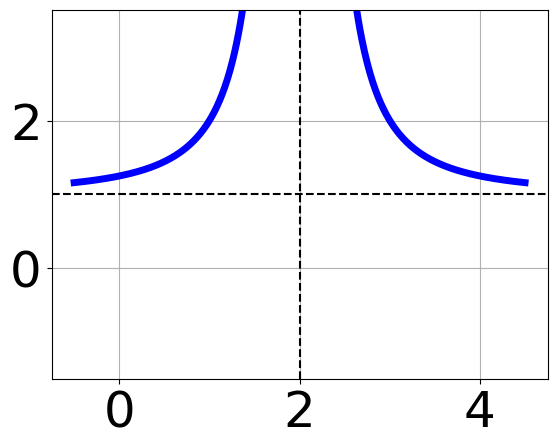
\includegraphics[width = 0.3\textwidth]{../Figures/rationalEquationToGraphCopyDC.png}\end{multicols}\item None of the above.
\end{enumerate} }
\litem{
Determine the domain of the function below.\[ f(x) = \frac{6}{15x^{2} -38 x + 24} \]\begin{enumerate}[label=\Alph*.]
\item \( \text{All Real numbers except } x = a, \text{ where } a \in [11.98, 12.15] \)
\item \( \text{All Real numbers.} \)
\item \( \text{All Real numbers except } x = a \text{ and } x = b, \text{ where } a \in [11.98, 12.15] \text{ and } b \in [29.98, 30.12] \)
\item \( \text{All Real numbers except } x = a, \text{ where } a \in [1.2, 1.24] \)
\item \( \text{All Real numbers except } x = a \text{ and } x = b, \text{ where } a \in [1.2, 1.24] \text{ and } b \in [1.31, 1.43] \)

\end{enumerate} }
\litem{
Solve the rational equation below. Then, choose the interval(s) that the solution(s) belongs to.\[ \frac{-8}{-5x + 2} + -9 = \frac{-9}{-45x + 18} \]\begin{enumerate}[label=\Alph*.]
\item \( x \in [-1.44,1.56] \)
\item \( x_1 \in [0.23, 0.43] \text{ and } x_2 \in [-0.44,3.56] \)
\item \( \text{All solutions lead to invalid or complex values in the equation.} \)
\item \( x \in [-0.37,-0.15] \)
\item \( x_1 \in [-0.37, -0.15] \text{ and } x_2 \in [-0.44,3.56] \)

\end{enumerate} }
\litem{
Choose the graph of the equation below.\[ f(x) = \frac{1}{x + 2} + 3 \]\begin{enumerate}[label=\Alph*.]
\begin{multicols}{2}\item 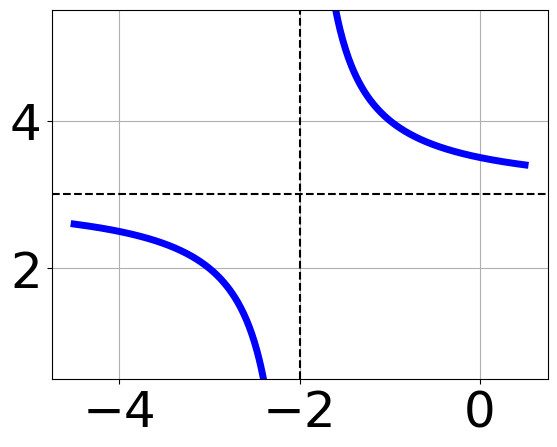
\includegraphics[width = 0.3\textwidth]{../Figures/rationalEquationToGraphAC.png}\item 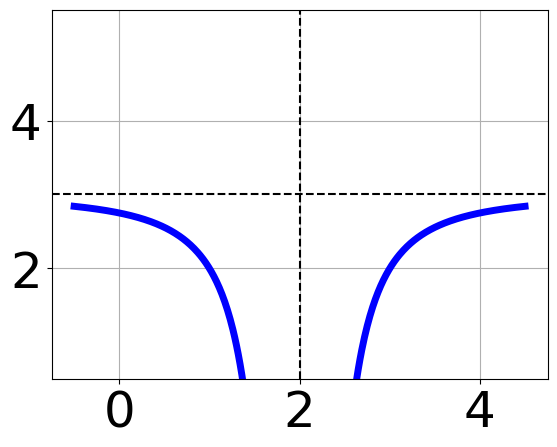
\includegraphics[width = 0.3\textwidth]{../Figures/rationalEquationToGraphBC.png}\item 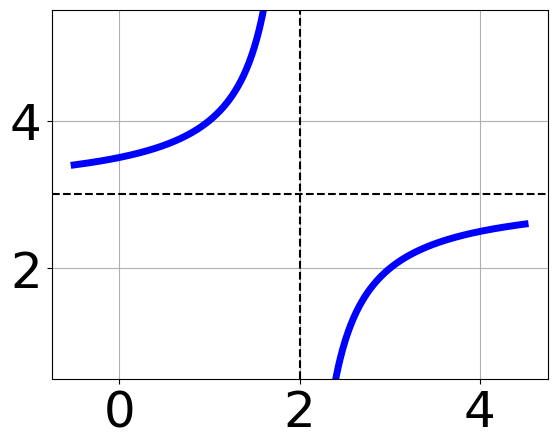
\includegraphics[width = 0.3\textwidth]{../Figures/rationalEquationToGraphCC.png}\item 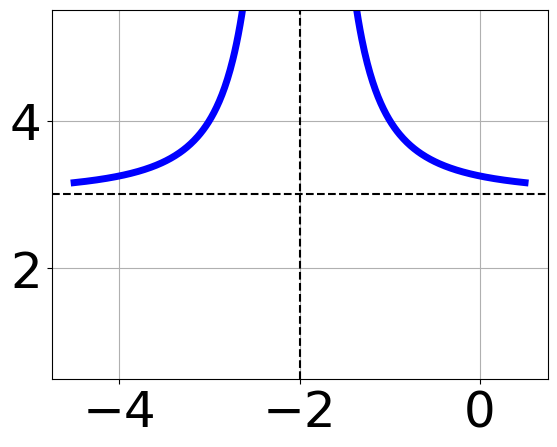
\includegraphics[width = 0.3\textwidth]{../Figures/rationalEquationToGraphDC.png}\end{multicols}\item None of the above.
\end{enumerate} }
\litem{
Choose the equation of the function graphed below.
\begin{center}
    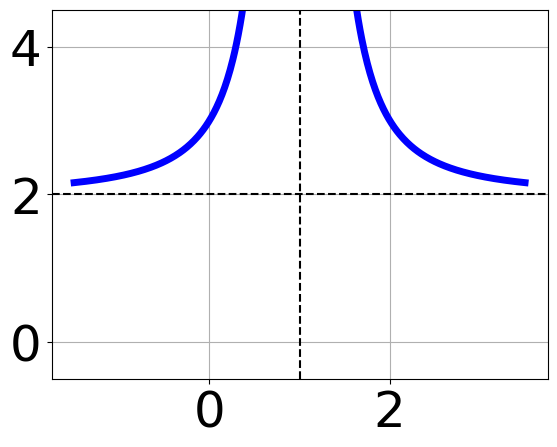
\includegraphics[width=0.5\textwidth]{../Figures/rationalGraphToEquationC.png}
\end{center}
\begin{enumerate}[label=\Alph*.]
\item \( f(x) = \frac{-1}{x - 1} + 0 \)
\item \( f(x) = \frac{1}{x + 1} + 0 \)
\item \( f(x) = \frac{-1}{(x - 1)^2} + 0 \)
\item \( f(x) = \frac{1}{(x + 1)^2} + 0 \)
\item \( \text{None of the above} \)

\end{enumerate} }
\litem{
Solve the rational equation below. Then, choose the interval(s) that the solution(s) belongs to.\[ \frac{-7x}{2x -7} + \frac{-7x^{2}}{10x^{2} -39 x + 14} = \frac{-4}{5x -2} \]\begin{enumerate}[label=\Alph*.]
\item \( x \in [-0.24,0.83] \)
\item \( \text{All solutions lead to invalid or complex values in the equation.} \)
\item \( x_1 \in [2.32, 5.4] \text{ and } x_2 \in [-0.04,0.83] \)
\item \( x_1 \in [0.7, 2.1] \text{ and } x_2 \in [-0.72,0.38] \)
\item \( x \in [2.32,5.4] \)

\end{enumerate} }
\litem{
Solve the rational equation below. Then, choose the interval(s) that the solution(s) belongs to.\[ \frac{-6x}{-5x + 4} + \frac{-4x^{2}}{-20x^{2} -4 x + 16} = \frac{-2}{4x + 4} \]\begin{enumerate}[label=\Alph*.]
\item \( x_1 \in [-0.08, 0.53] \text{ and } x_2 \in [-1.2,6.8] \)
\item \( x \in [-1.06,-0.81] \)
\item \( \text{All solutions lead to invalid or complex values in the equation.} \)
\item \( x \in [-1.47,-1.3] \)
\item \( x_1 \in [-0.08, 0.53] \text{ and } x_2 \in [-1.42,0.58] \)

\end{enumerate} }
\end{enumerate}

\end{document}